\documentclass[11pt,twoside,a4paper]{report}
\usepackage{polski}
\usepackage[utf8]{inputenc}
\usepackage{graphicx}
\usepackage{wrapfig}

% Title Page
\title{Użycie języka Swift i elementów paradygmatu reaktywnego na przykładzie aplikacji mobilnej do polecania filmów i seriali}
\author{Bartosz Woliński}

\begin{document}
\maketitle
\tableofcontents
\chapter{WSTĘP}

\paragraph{}Motywacją do powstania pracy inżynierskiej o tej tematyce, była chęć poznania i zrozumienia idei paradygmatu reaktywnego w programowaniu na platformę mobilną. W mojej pracy postaram się pokazać, że podejście reaktywne jest dobrym pomysłem szczególnie w środowiskach oferujących niewielkie zasoby. Co prawda dzisiejsze smartfony posiadają coraz wydajniejsze procesory i coraz szybsze pamięci RAM, jednakże nadal nie są to komponenty tak sprawne jak te używane w komputerach klasy PC. Z tego powodu uważam, że zrównoleglanie procesów i obliczeń ma sens na platformach mobilnych a w tym celu warto pochylić się nad paradygmatem reaktywnym.\\ Po raz pierwszy ideę programowania reaktywnego zaproponowała firma Microsoft tworząc framework Reactive Extensions na platformę .NET i opierając go głównie o popularny wzorzec obserwatora.\cite{MicrosoftRx} 
Używany termin programowanie reaktywne odnosi się do programowania reaktywnego funkcyjnego jako, że te dwa pojęcia są ze sobą nierozerwalnie związane.
\subparagraph{}Celem programowania reaktywnego jest przede wszystkim bardziej efektywne podejście do celu i sensu działania aplikacji w ogólnym ujęciu a nie skrupulatne skupienie się na tym w jaki sposób konkretne zadania powinny być realizowane. Na takie podejście można sobie pozwolić, jako że programowanie reaktywne wymusza na systemie jego bezstanowość. Jest to możliwe m.in. dzięki temu, że programując w sposób reaktywny, działamy na strumieniach niezmiennych i niemodyfikowalnych danych w czasie a nie na pojedynczych zdarzeniach. Ponadto takie podejście pozwala oszczędzić dużo kodu i rozważań nad sensownością wydarzeń w czasie m.in dlatego, że zdarzenia synchroniczne jak i asynchroniczne traktowane są w ten sam sposób co znacząco ułatwia tworzenie logiki programu. Podstawą paradygmatu reaktywnego jest wzorzec obserwatora czyli wzorzec obiektu obserwowanego (nadawcy zdarzeń) i obiektu obserwującego (reagującego na odebrane zdarzenia).
\chapter{CEL I ZAKRES PRACY}
\paragraph{}Niniejsza praca dyplomowa składa się z dwóch zasadniczych części.\\Pierwsza z nich ma na celu podejście od strony teoretycznej do treści tematu. Rozumiem przez to objaśnienie idei paradygmatu reaktywnego i pojęć z nim związanych.\\Druga część pracy ma za zadanie przedstawienie praktycznego podejścia do tematu i zaprezentowanie sposobu użycia paradygmatu reaktywnego na przykładzie aplikacji mobilnej. Zadaniem tej aplikacji jest umożliwienie użytkownikowi wyszukania filmu lub serialu przy użyciu internetu i publicznego API OMDB. Znaleziony film lub serial może zostać zapisany w lokalnej bazie aplikacji. Projekt ma na celu ułatwienie decyzji użytkownikowi na temat tego co ma obejrzeć posiadając zadaną ilość czasu. Z pośród zapisanych filmów i seriali zaproponowane zostaną te spełniające wymagania czasowe. Po obejrzeniu danej produkcji, użytkownik będzie mógł ją ocenić a ocena ta również będzie zapisywana w lokalnej bazie.\\
Podsumowując powyższe stwierdzenia, przedstawiam zagadnienia opisane w obu częściach ninejszej pracy:
\subparagraph{Część teoretyczna:}
\begin{itemize}
	\item Krótka historia systemu iOS
	\item Użyty język programowania
	\item Istotne zagadnienia z tematu programowania funkcyjnego
	\item Opis zagadnień związanych z paradygmatem reaktywnym, t.j.: operatory reaktywne; współbieżność; wady i zalety tego podejścia
\end{itemize}
\subparagraph{Część opisująca pracę własną:}

\begin{itemize}
	\item Opis czynności przygotowawczych
	\item Zdefiniowanie wymagań funkcjonalnych i niefunkcjonalnych
	\item Opis modelu bazodanowego i zależności między klasami
	\item Charakterystyka użytych bibliotek i frameworków
	\item Implementacja aplikacji w środowisku XCode z wykorzystaniem języka Swift i opisem zastosowanej architektury
\end{itemize}

\chapter{ŹRÓDŁA I DEFINICJE}
\section{Historia i charakterystyka systemu iOS}
\paragraph{}iOS to mobilny system operacyjny stworzony przez firmę Apple Inc. na urządzenia iPod, iPhone i iPad. Został zaprezentowany w styczniu 2007 roku na konferencji Macworld. Jest jednym z dwóch\footnote{dane firmy Gartner Inc. za rok 2015: urządzenia mobilne z systemem android - 1,3 mld \\ urządzenia z systemem iOS - 297 milionów} najpopularniejszych systemów mobilnych. 
\paragraph{Specyfikacje techniczne}
\subparagraph{}System iOS oparty jest na jądrze systemu Darwin. Jest to unixowy system operacyjny typu open-source wypuszczony przez Apple Inc. w 2000 roku. Zbudowany jest w oparciu o projekty firm Apple, NeXTSTEP, BSD, Mach i kilka innych. System działa na architekturach PowerPC, Intel x86 i ARM.\cite{pureDarwin}\cite{openGroup} 
Jądrem systemu Darwin jest XNU. Jest to hybrodowe jądro łączące w swojej implementacji Mach 3 microkernel i elementy BSD t.j. stos sieciowy czy wirtualny system plików.\cite{XNUkernel}
\paragraph{Wersje systemu iOS}
\subparagraph{iPhone OS -}pierwsza iteracja mobilnego systemu Apple. Nie nadano żadnej oficjalnej nazwy. Jedyne co utrzymywano to, że iPhone korzysta z jednej z desktopowych wersji systemu OSX.\cite{iphoneOSX} 
W marcu 2008 roku wypuszczono zestaw narzędzi do programowania na tę platformę: iPhone SDK \cite{iphoneSDK}
\subparagraph{iPhone OS 2.0 -}w lipcu 2008 roku, wraz z premierą urządzenia iPhone 3G, miała miejsce premiera systemu iPhone OS 2.0. Najistotniejszą usługą jaką wprowadzał ten system był sklep App Store. Dzięki niemu programiści mogli rozpocząć rozprowadzanie swoich aplikacji na urządzenia iPhone i iPod Touch. \cite{iphone3GappStore}
\subparagraph{iPhone OS 3.0 -}Odświeżony smartfon Apple iPhone3GS został wypuszczony wraz z nowym systemem - iPhone OS 3.0. Jego najbardziej rozpoznawalną cechą było wprowadzenie czegoś co dziś w każdym systemie mobilnym musi być i jest oczywiste. Chodzi o funkcje kopiowania i wklejania, bez których nie wyobrażamy sobie systemu operacyjnego. Ponadto dostarczał funkcjonalności takich jak: Spotlight Search, klawiatura w układzie horyzontalnym i możliwość wysyłania wiadomości MMS.\cite{iphoneOS3}
\subparagraph{iOS 4 -}Pierwszy system o tej nazwie, wprowadzony na rynek w kwietniu 2010 roku. Wówczas Apple zaprezentowało urządzenie iPhone 4 oraz zrezygnowało ze wsparcia urządzeń iPhone i iPod Touch. Wraz z premierą nowego systemu, firma oddała do dyspozycji około 1500 API dla programistów. Najistotniejszym z nich było to obłusugujące multitasking, wprowadzony po raz pierwszy w mobilnych systemach Apple. Multitasking pozwalał użytkownikom na m.in. przełączanie się między aplikacjami działającymi w tyle za pomocą podwójnego kliknięcia przycisku home. Poprzednie urządzenia ze względu na swoją architekturę nie pozwalały na to.\cite{ios4}
\subparagraph{iOS 5 -}W październiku 2011 swoją premierę miał iPhone 4s - urządzenie z dwurdzeniowym procesorem - a wraz z nim system iOS 5. Nowy system oferował takie usługi jak Siri (asystent głosowy), iMessage (system wiadomości oparty o połączenie internetowe), synchronizacja z iCloud czy Notification Center. Bardzo istostny z punktu widzenia programistów, ponieważ oferuje on możliwość tworzenia i wysyłania powiadomień od aplikacji do systemu i wyświetlania ich w górnym pasku.\cite{ios5}
\subparagraph{iOS 6 -}Po raz pierwszy zaprezentowany w czerwcu 2012 roku. Wraz z nowym urządzeniem - iPhonem 5 - miał wprowadzać kilka udogodnień. Były to między innymi: kompletnie odświeżona aplikacja map i nawigacji GPS, która uwzględniała ruch uliczny. Ponadto dostarczono pełną integrację z systemem Facebook oraz usługę FaceTime - wideorozmowy za pośrednictwem telefonii komórkowej.\cite{ios6}
\subparagraph{iOS 7 -}Najbardziej znaczący update systemu iOS wg Craiga Federighi'ego.\footnote{Wiceprzewodniczący działu inżynierii oprogramowania Apple} Zaprezentowany w czerwcu 2013 roku. System zaprezentował kompletnie odświeżony interfejs użytkownika. Najważniejszą funkcjonalnością był Control Center czyli zestaw najczęściej używanych opcji obsługiwany przez wysunięcie za pomocą paska od dołu ekranu. Ponadto wszelkie notyfikacje systemu były wyświetlane również na zablokowanym ekranie urządzenia. Oprócz tego nowy system dostarczył wiele nowych API dla programistów, w tym ulepszony multitasking, dzięki któremu aplikacje mogły wykonywać wiele operacji w tle. Poza powyższymi, iOS 7 wprowadził jeszcze jedną istotną usługę - AirDrop czyli nowy sposób przesyłania danych między użytkownikami w sposób zaszyfrowany, korzystając z połączenia typu peer-to-peer.\cite{ios7}
\subparagraph{iOS 8 -}Największy dotychczasowy zestaw 4000 nowych API został zaprezentowany wraz z systemem iOS 8 w czerwcu 2014 roku. Zestaw ten obejmował całkowicie nowy język programowania na platformę jakim jest Swift. iOS 8 wprowadzał następujące nowości: widgety Notification Center, klawiatury dostępne z poziomu zewnętrznych aplikacji, HealthKit - system zdrowotny pomagający użytkownikowi w przechowywaniu i analizowaniu parametrów stanu zdrowia, HomeKit - aplikacja do integracji z systemami typu smart house. Wraz z prezentacją urządzenia iPhone 6 z procesorem A7, pojawił się również nowy silnik graficzny - Metal, w pełni wykorzystujący nową architekturę urządzenia do tworzenia gier i animacji.\cite{ios8}
\subparagraph{iOS 9 -}Czerwiec 2015 roku był datą pierwszej publicznej prezentacji systemu iOS 9. Na urządzeniach iPad wprowadzono funkcję używania dwóch aplikacji jednocześnie w trybie side-by-side i Picture-in-Picture. Ponadto, ulepszono Mapy uwzględniając nawigację przy użyciu publicznego transportu. Oprócz tego system wprowadził kilka optymalizacji pozwalających na dłuższy czas pracy na baterii. Jeśli chodzi o narzędzia dla programistów to stworzono nowy framework do produkcji gier - GameKit. Wprowadzono również usługę CarPlay, bardzo istotną dla producentów samochodów. Dzięki niej możliwe jest sparowanie urządzenia z systemem pojazdu i wywoływania funkcji. Ponadto swoją premierę miała druga implementacja języka Swift czyli Swift 2.0 oraz stał się projektem open source.\cite{ios9}
\subparagraph{iOS 10 -}Ostatnia opisywana przeze mnie iteracja systemu iOS ujrzała światło dzienne w czerwcu 2016 roku. Według Craiga Federighi'ego jest to największe i najbardziej znaczące wydanie iOS'a. Istotne nowości wprowadzone przez system to m.in. otwarcie API wiadomości dla programistów, otwarcie API Siri, kompletny redesign aplikacji Mapy, nowy design Apple Music, obsługa 3D touch dla urządzeń iPhone 6 i nowszych. W tym samym roku premierę ma kolejna implementacja języka Swift - Swift 3.0 będąca bardziej kompatybilną wstecznie z językiem Objective-C.\cite{compatibility}\cite{ios10}
\section{Historia i charakterystyka języka Swift}
\paragraph{}Swift to kompilowany, hybrydowy język programowania stworzony przez firmę Apple Inc. Jego premiera odbyła się podczas Worldwide Developers Conference w czerwcu 2014 roku.\cite{swiftHistory} 
\paragraph{}Jeden z twórców \footnote{Chris Lattner - inżynier Apple} opisuje Swifta jako narzędzie czerpiące idee z wielu innych języków t.j. Objective-C, Rust, Haskell, Ruby, Python, C\#, CLU i wielu innych. 
\paragraph{}Swift został stworzony jako nowoczesny następca Objective-C na platformy MacOS i iOS, ale w grudniu 2015 roku stał się językiem open source. Oznacza to, że została stworzona społeczność przy użyciu serwisu Swift.org a oprócz tego udostępniono publiczne repozytorium Gita. Ponadto uwolniono narzędzia takie jak kompilator LLVM, biblioteki standardowe czy menedżer zależności projektu. Dodatkowo Swift otrzymał wsparcie na platformę Linux.\cite{swiftOpensource}
\paragraph{Główne różnice między Swiftem a Objective-C}
\subparagraph{}Swift jako język mający na celu zastąpienie leciwego już Objective-C, oferuje wiele nowych mechanizmów.
\subparagraph{Wartości opcjonalne - } pozwalają funkcjom, które nie zawsze zwrócą konkretną wartość lub obiekt na zwrócenie obiektu enkapsulowanego w wartość opcjonalną bądź wartość nil. W języku C i Objective-C funkcje mogą zwrócić wartość pustą (nil) nawet jeżeli spodziewana wartość jest typu stuktury lub klasy. W Objective-C zwrócenie przez funkcję wartości pustej (pomimo innej spodziewanej) nie powoduje błędów kompilacji ani błędów w czasie działania. W Swficie zaś w takiej sytuacji mielibyśmy do czynienia z błędem kompilacji lub błędem krytycznym w czasie działania co chroni nas przed niespodziewanymi zachowaniami.
\subparagraph{Wnioskowanie typów - } kompilator języka Swift jest w stanie wywnioskować typ tworzonej zmiennej. Ponadto zmienna o zadeklarowanym (wywnioskowanym) typie nie może go zmienić.
\subparagraph{Krotki - } Swift wspiera obiekty krotkowe, czyli takie, które mogą przechowywać na raz kilka wartości różnych typów. Dzięki temu możliwe jest zwracanie przez funkcji wielu wartości.
\subparagraph{Guard - } wyrażenie warunkowe w składni Swifta. Zapewnia weryfikacje poprawności oczekiwanego typu zmiennej a w razie błędu, może spowodować wcześniejsze wyjście z funkcji.
\subparagraph{Elementy programowania funkcyjnego - } Swift posiada możliwość programowania funkcyjnego co niejednokrotnie jest dużo bardziej czytelne i wydajne od tradycyjnego podejścia. Z tego powodu oferuje on operatory funkcyjne typu \textbf{map} czy \textbf{filter}.       
\subparagraph{Enumeratory - } W Swficie, podejście do enumeratorów zostało bardzo rozbudowane. Mogą one zawierać metody i być przekazywane przez wartość.
\subparagraph{Podejście do funkcji - } Każda funkcja w Swifcie posiada typ, który składa się z typów parametrów oraz typu zwracanego. To oznacza, że można przypisywać funkcje do zmiennych a nawet przesyłać je jako parametry innych funkcji.
\subparagraph{Słowo kluczowe "do" - } pozwala na utworzenie nowego zakresu w kodzie a ponadto może zawierać mechanizm obsłusgi błędów, znany z innych jęzków t.j. "try catch". \cite{swiftObjcDiff}
\section{Paragydmat funkcyjny}
\section{Paragydmat reaktywny}
\paragraph{}Programowanie reaktywne funkcyjne ma swoje początki już w roku 1997\cite{beginningOfRx} lecz popularne stało się za sprawą firmy Microsoft i biblioteki Reactive Extensions dla platformy .NET z 2009 roku\cite{rxMicrosoftYear}.\\
Najczęściej podczas tworzenia programu, oczekuje się, że instrukcje będą wykonywane stopniowo, po jednej na raz, w kolejności w jakiej zostały napisane. W przypadku programowania reaktywnego, wiele instrukcji może wykonywać się współbieżnie a ich wyniki przechwytywane są w późniejszym czasie, w losowej kolejności przez tak zwanych obserwatorów (ang. observer). Zamiast wywoływania metody, defniuje się mechanizm odszukiwania i przekształcania danych, w formie tak zwanego obiektu obserowanego (ang. observable) a następnie zasubskrybowuje się (rozpoczyna nasłuchiwanie) obserwatora do tego obiektu. Na tym etapie uprzednio zdefiniowany mechanizm rozpoczyna działanie z obserwatorem będącym swego rodzaju strażnikiem, gotowym na przechwycenie i odpowiedź na emitowane zdarzenia.\\
Niewątpliwą zaletą takiego podejścia jest możliwe współbieżne wykonywanie wielu niezależnych od siebie zadań. W ten sposób czas wykonania wszystkich tych zadań będzie mniej więcej równy czasowi wykonania najdłuższego z nich.
\subsection{Idea programowania reaktywnego}
\paragraph{}Podstawowym założeniem podejścia reaktywnego jest programowanie oparte o asynchroniczne strumienie (sygnały) niemodyfikowalnych danych.\\
Źródłem sygnałów mogą być dowolne zdarzenia w czasie takie jak: modyfikacja zmiennych, interakcja użytkownika, pozycja kursora, struktury danych, zapytania sieciowe, operacje bazodanowe itp. Dane otrzymywane ze strumienia są przetwarzane przez obserwatora i na tej podstawie podejmowane są decyzje i skutki uboczne.\\
Sygnały w programowaniu reaktywnym mogą zostać scharakteryzowane ze względu na sposób działania, na dwie grupy: sygnały "zimne" i sygnały "gorące".
\subparagraph{Sygnał gorący} zużywa zasoby i emituje zdarzenia bez względu na to czy istnieje zasubskrybowany do niego obserwator. Zdarzeniami są tutaj najczęściej dane o informujące o modyfikacji zmiennych lub obiektów, koordynaty kliknięć lub kursora myszy, informacje o kliknięciach w kontrolki UI, bieżący czas, itp. Jak widać są to raczej sygnały ciągłe i posiadające zwykle więcej niż jedną daną w sekwencji. Nie ma zatem sensu mówienie o końcu ciągu zdarzeń w tym sygnale. Ponadto kolejno emitowane dane powielane są do wszystkich nasłuchujących.
\subparagraph{Sygnał zimny} nie zużywa zasoboów ani nie emituje zdarzeń dopóki obserwator nie zacznie nasłuchiwać na zmiany. Zdarzeniami najczęściej są tutaj operacje asynchroniczne, połączenia HTTP, połączenia TCP, połączenia strumieniowane. Zwykle w swojej sekwencji zawiera jedno zdarzenie będące np. wynikiem odpytania sieciowego. Ponadto wyemitowany wynik najczęściej kierowany jest to jednego obserwującego.
\subparagraph{Subskrybcja -}za pomocą operatora subskrybcji, w programowaniu reaktywnym, łączony jest obiekt obserwowany i obserwator. Aby obiekt nasłuchujący mógł odbierać nadawane sygnały lub odebrać nadany błąd, musi najpierw zasubskrybować się do obiektu obserwowanego. Typowa implementacja operatora subskrybcji operuje na poniższych trzech metodach:
\begin{itemize}
	\item onNext: nasłuchiway obiekt wywołuje tę metodę, gdy tylko wyemituje zdarzenie. Parametrem tej metody jest emitowane zdarzenie.
	\item onError: obserwowany obiekt wywołuje tę metodę, aby powiadomić o niepowodzeniu przy generowaniu oczekiwanych danych lub o napotkaniu innego błędu. Zatrzymuje to działanie obserwowanego i przerywa kolejne wywołania metody onNext lub onCompleted. Metoda onError, jako parametr, powinna przyjmować obiekt reprezentujący napotkany błąd.
	\item onCompleted: obserwowany wywołuje tę metodę po ostatnim wywołaniu metody onNext, jeżeli nie napotkano błędu.
\end{itemize}
\begin{figure}[ht!]
\centering
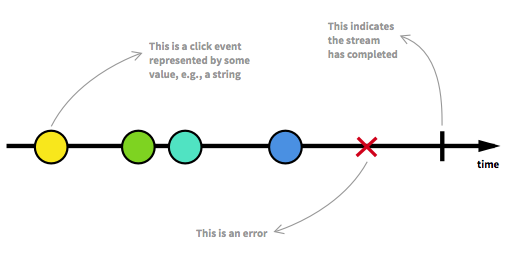
\includegraphics[width=10cm]{sygnalRx}
\caption{Schemat emitowanych danych w sygnale}
\label{sygnalRx}
\end{figure}
Jak widać na powyższym obrazku, sygnał jest ciągiem poszeregowanych zdarzeń w czasie. Przechwytywanie powyższych zdarzeń odbywa się asynchronicznie a każdy z wymienionych stanów sygnału musi być obsłużony przez zdefiniowane w tym celu funkcje. \\
\subparagraph{Obiekty Subject -} stanowią w programowaniu reaktywnym swego rodzaju most, w większości implementacji podejścia reaktywnego, ponieważ zachowują się jednocześnie jak obiekty obserwowane i obserwujące. Jako obserwatorzy, mogą zasubskrybować się do jednego lub więcej obserwowanych obiektów. Jako obserwowani mogą emitować i reemitować zdarzenia do obiektów obserwujących.\\
Rozróżnia się cztery rodzaje obiektów Subject zaprojektowanych pod konkretne przypadki.  
\subparagraph{AsyncSubject -} emituje ostatnią (i tylko ostatnią) wartość wyemitowaną przez źródołwy sygnał i tylko, gdy źródłowy sygnał zakończy się poprawnie. Jeśli źródłowy obiekt obserwowany zakończy się nie emitując żadnych wartości, obiekt AsyncSubject również zakończy się nie emitując żadnych wartości.
\begin{figure}[ht!]
	\centering
	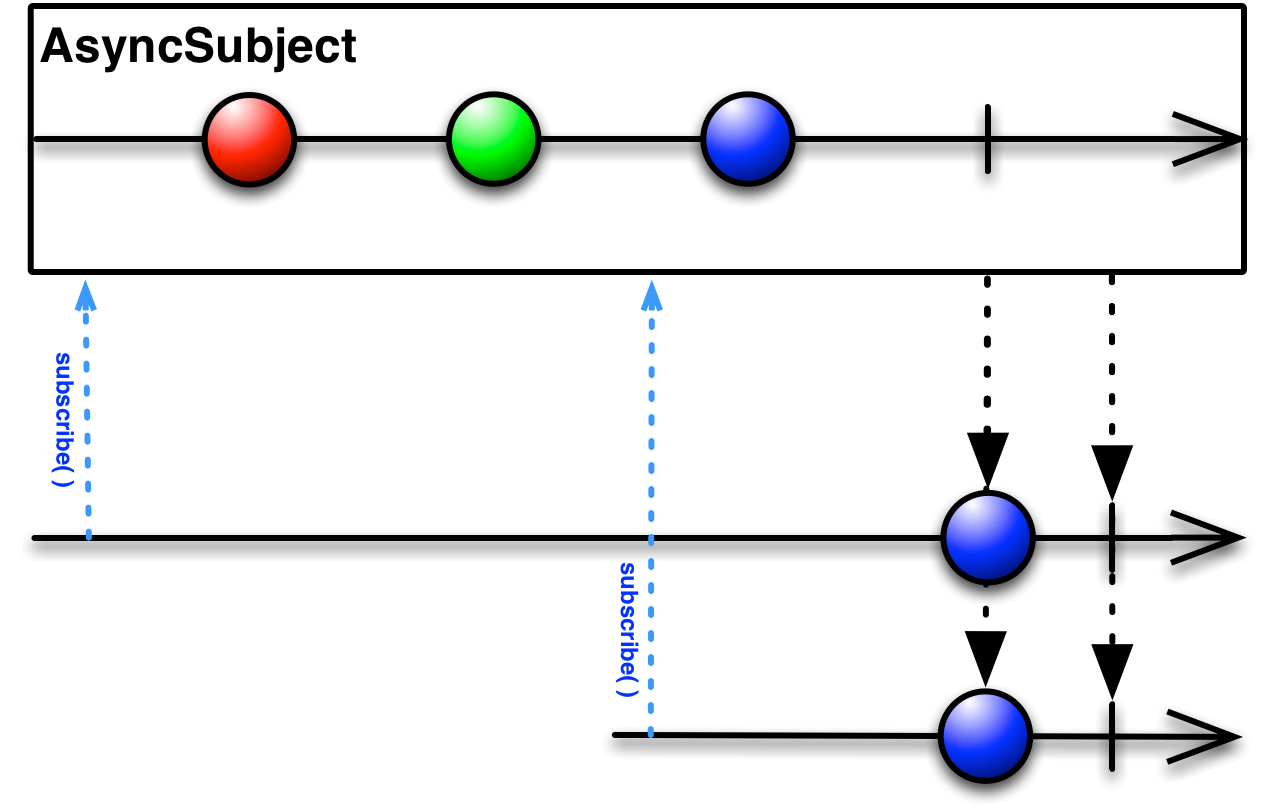
\includegraphics[width=10cm]{asyncSubject}
	\caption{Schemat poprawnie zakończonego działania obiektu AsyncSubject}
	\label{asyncSubject}
\end{figure}
\\
\\

Jeśli zaś źródłowy sygnał zakończy się błędem, obiekt AsyncSubject nie wyemituje żadnych wartości lecz informacje o błędzie od sygnału źródłowego.
\begin{figure}[ht!]
	\centering
	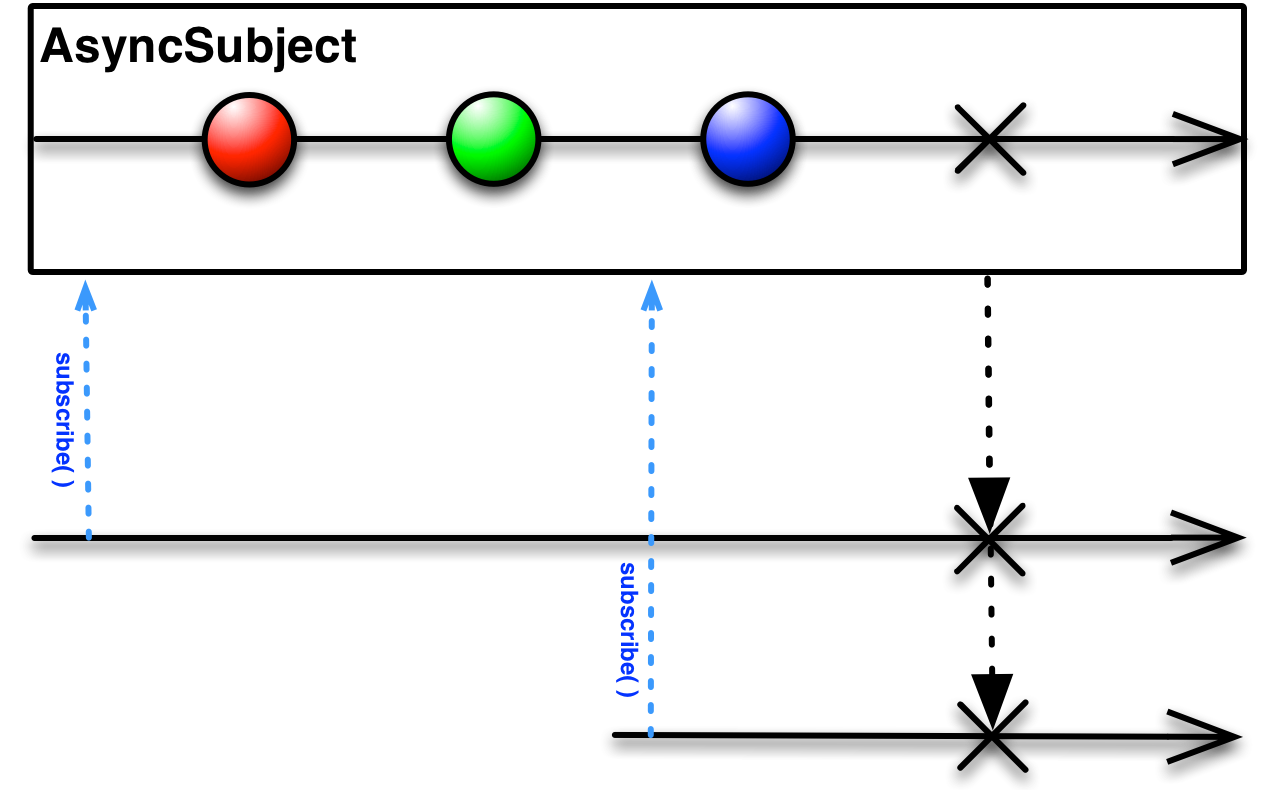
\includegraphics[width=10cm]{asyncSubjectFailed}
	\caption{Schemat działania obiektu AsyncSubject w przypadku błędu}
	\label{asyncSubjectFailed}
\end{figure}
\subparagraph{BehaviorSubject -}gdy obserwator zasubskrybuje się do obiektu BehaviorSubject, rozpoczyna on emitowanie zdarzeń rozpoczynając od ostatniego uprzednio wyemitowanego przez źródłowy sygnał a następnie kontynuuje emitowanie kolejnych zdarzeń sygnału źródłowego.
\begin{figure}[ht!]
	\centering
	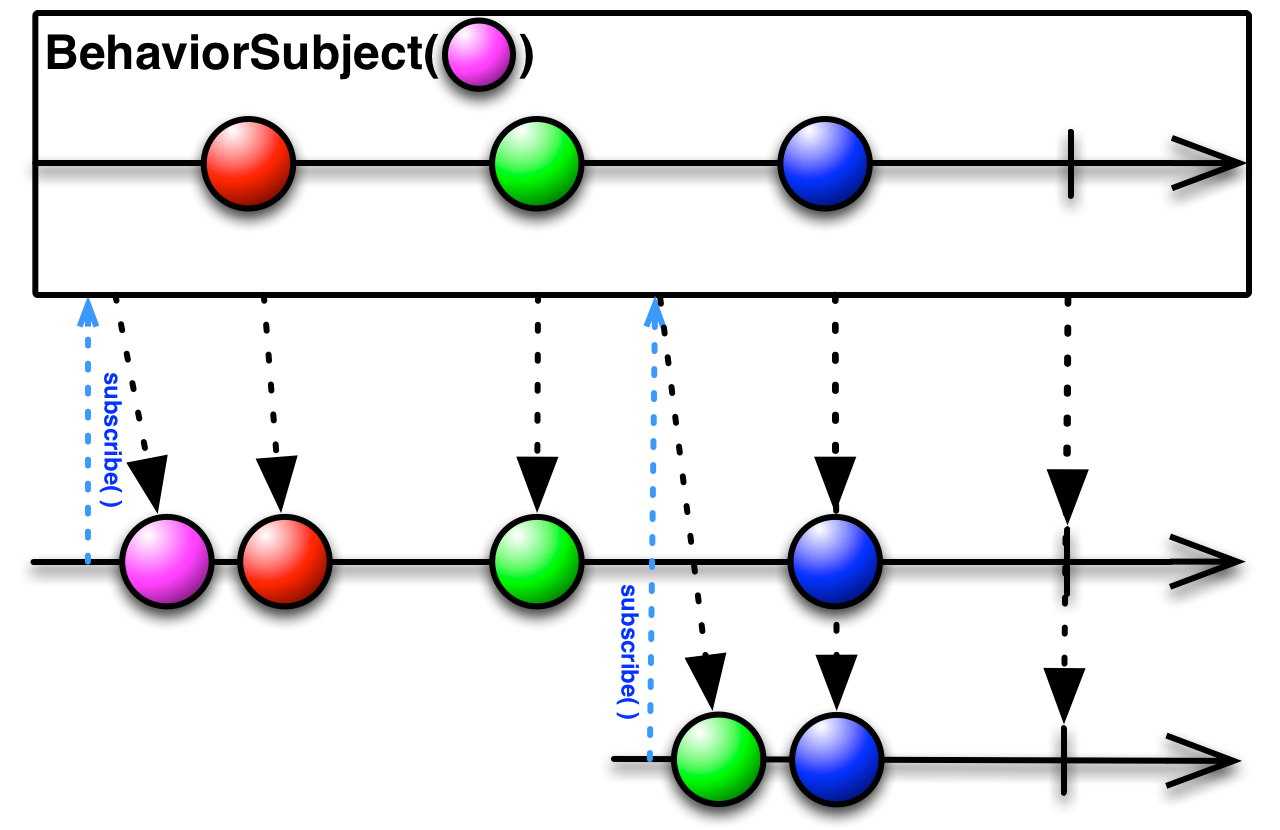
\includegraphics[width=10cm]{behaviorSubject}
	\caption{Schemat działania obiektu BehaviorSubject}
	\label{behaviorSubject}
\end{figure}
\\
\\
\\
Jeśli zaś źródłowy sygnał zakończy się błędem, obiekt BehaviorSubject nie wyemituje żadnych danych do kolejnych obserwatorów, lecz prześle informacje o błędzie z obiektu źródłowego.
\begin{figure}[ht!]
	\centering
	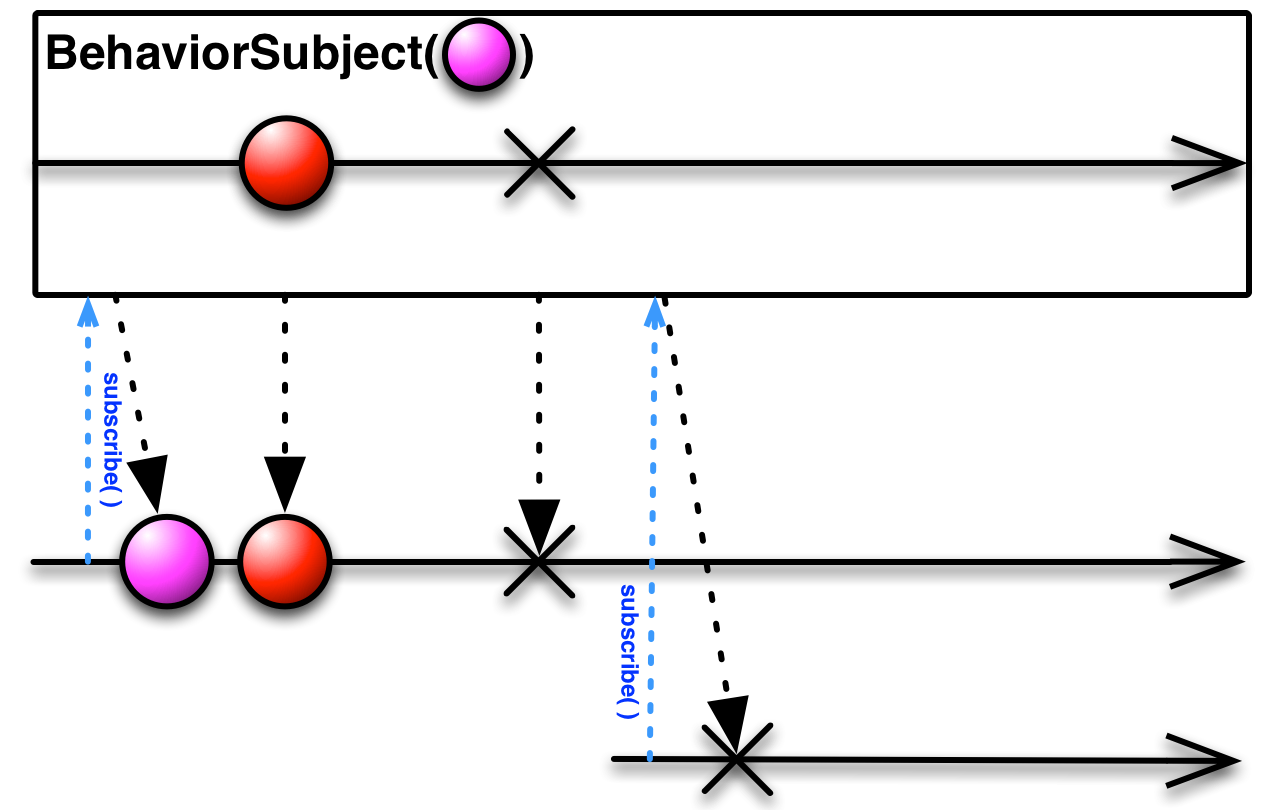
\includegraphics[width=10cm]{behaviorSubjectFailed}
	\caption{Schemat działania obiektu BehaviorSubject w przyadku błędu}
	\label{behaviorSubjectFailed}
\end{figure}
\subparagraph{PublishSubject -}emituje do obserwatora wszystkie dane wyemitowane od momentu subskrypcji. Obiekt PublishSubject może rozpocząć emitowanie danych bezpośrednio po utworzeniu. Istnieje zatem ryzyko, że jedno lub więcej wyemitowanych zdarzeń może zostać zgubiona od czasu powstania obiektu Subject i obserwatora subskrybującego się do niego. Aby temu zapobiec, można przekształcić sygnał w "zimny" przez manualne użycie funkcji Create i upewnienie się, że zdarzenia nie są emitowane dopóki wszyscy obserwatorzy sie nie zasubskrybują. 
\begin{figure}[ht!]
	\centering
	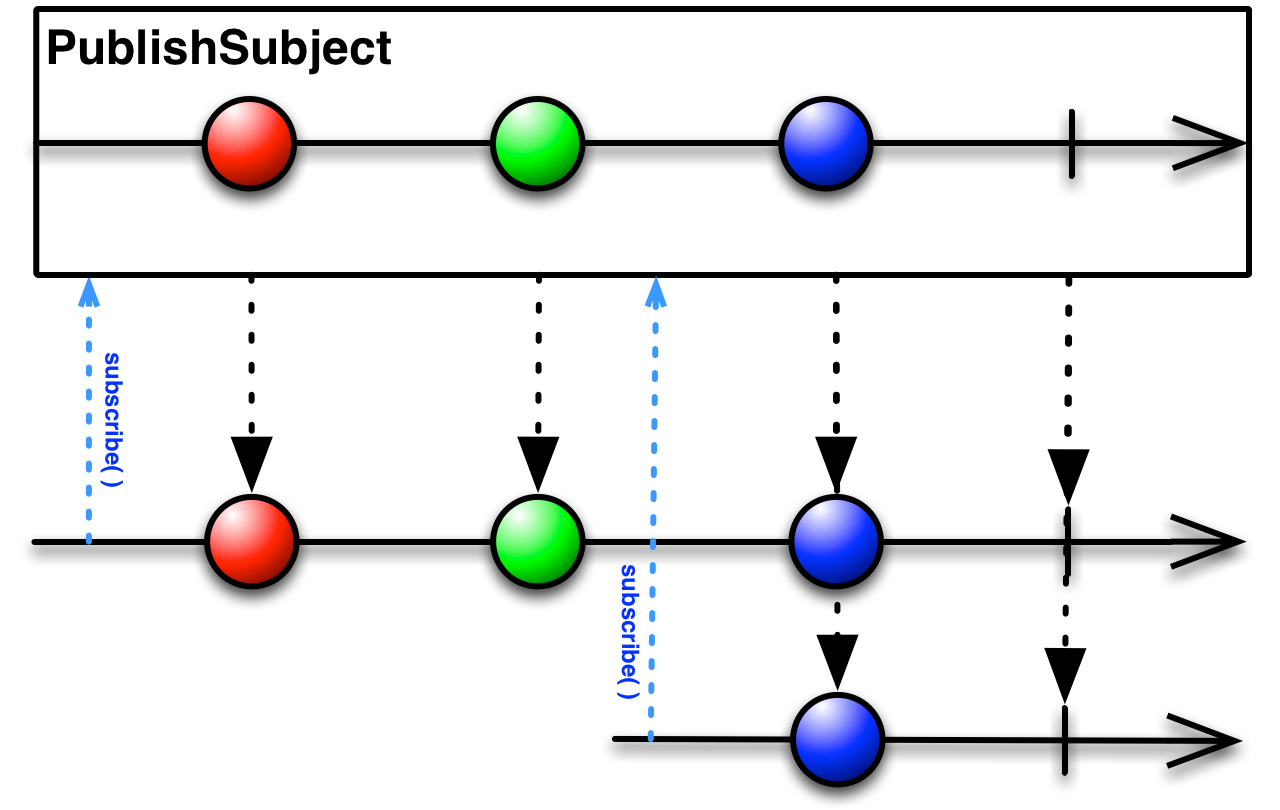
\includegraphics[width=10cm]{publishSubject}
	\caption{Schemat działania obiektu PublishSubject}
	\label{publishSubject}
\end{figure}
\\
\\
Jeśli zaś źródłowy sygnał zakończy się błędem, obiekt PublishSubject nie wyemituje danych, lecz prześle informacje o błędzie z obiektu źródłowego.
\begin{figure}[ht!]
	\centering
	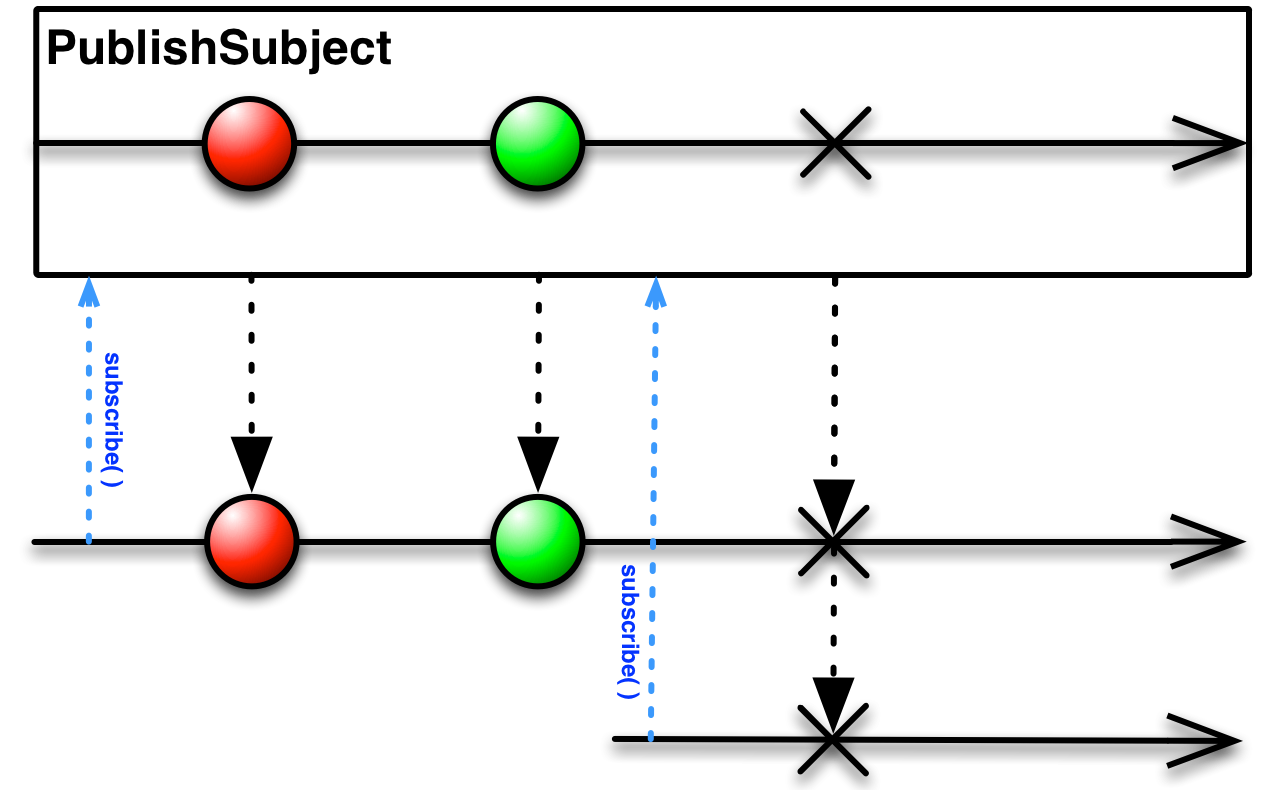
\includegraphics[width=10cm]{publishSubjectFailed}
	\caption{Schemat działania obiektu PublishSubject w przypadku błędu}
	\label{publishSubjectFailed}
\end{figure}
\subparagraph{ReplaySubject -}emituje do obserwatorów wszystkie zdarzenia wyemitowane przez sygnał źródłowy, bez względu na moment subskrypcji. 
\begin{figure}[ht!]
	\centering
	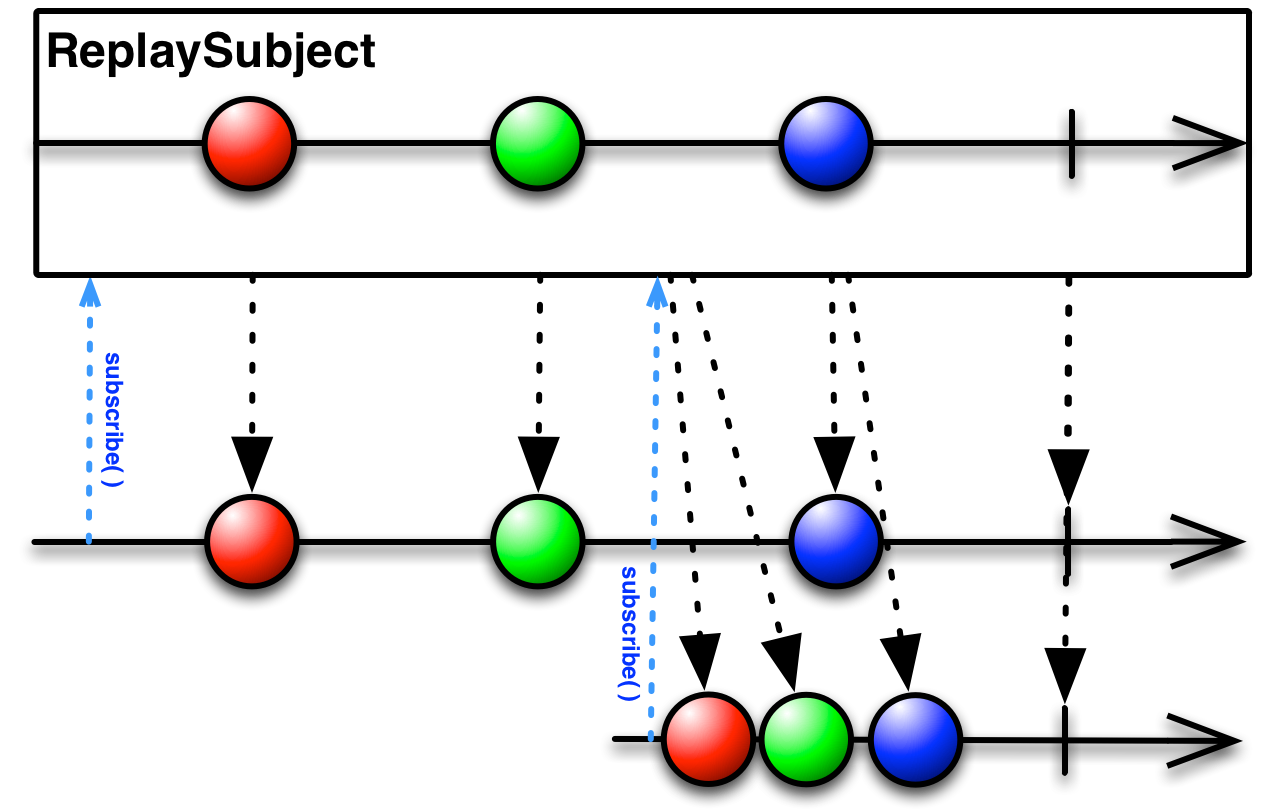
\includegraphics[width=10cm]{replaySubject}
	\caption{Schemat działania obiektu ReaplySubject}
	\label{replaySubject}
\end{figure}\\
Możliwa jest implementacja obiektu ReplaySubject, której działanie będzie polegało na odrzuceniu starych zdarzeń, czyli obostrzonych rozmiarem bufora bądź upływem zadanej ilości czasu.\\
Obiekt ReplaySubject używany jako obserwator, dba o to by jego metoda onNext (lub inne metody on) nie były wywoływane z różnych wątków. Może to doprowadzić do powielania już raz wyemitowanych zdarzeń i niejednoznaczności, co stoi w sprzeczności z wytycznymi projektowymi paradgymatu reaktywnego.\cite{rxDesignGuideline} 
\subsection{Podejście reaktywne w praktyce}
\subsection{Operatory reaktywne}
\paragraph{}Znaczna część operatorów reaktywnych została zaczerpnięta z podejścia funkcyjnego. Mają na celu umożliwienie tworzenia sygnałów, przekształcania w inne, filtrowania, łączenia, obsługi błędów, itp.\\
Większość operatorów programowania reaktywnego działa na obiekcie typu Observable a wynikiem działania jest obiekt typu Observable. Dlatego stosowane jest podejście łączenia operacji w całe łańcuchy działań na sygnałach. Należy tu jednak podkreślić, że kolejne operatory łańcucha nie działają na oryginalnym obiekcie Observable niezależnie. Operują one kolejno na wynikach poprzednich działań w łańcuchu czyli na kolejnych obiektach Observable. \\
W dalszej części tego paragrafu zostaną scharakteryzowane najczęściej stosowane operatory reaktywne.
\paragraph{Operatory tworzenia sygnałów}
\subparagraph{Create -}tworzy od podstaw obiekt Observable. Do operatora podawana jest funkcja przyjmująca w argumencie obiekt obserwującego. Tworzy się za jej pomocą obiekt obserwowany, przez zdefniowanie działań funkcji onNext, onError i onCompleted. 
\begin{figure}[ht!]
	\centering
	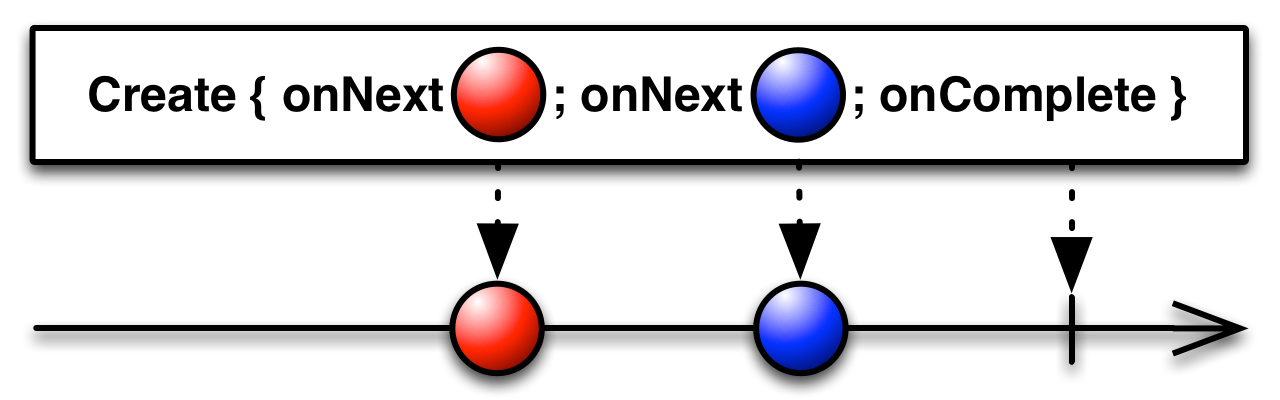
\includegraphics[width=6cm]{create}
	\caption{Schemat działania operatora Create}
	\label{create}
\end{figure}\\
\subparagraph{Defer -}tworzy obiekt Observable, ale dopiero gdy obserwator się do niego zasubskrybuje. Działanie to jest powielane dla każdego subskrybenta, dlatego, pomimo iż wszyscy nasłuchują z tego samego sygnału, otrzymują indywidualne sekwencje zdarzeń. 
\begin{figure}[ht!]
	\centering
	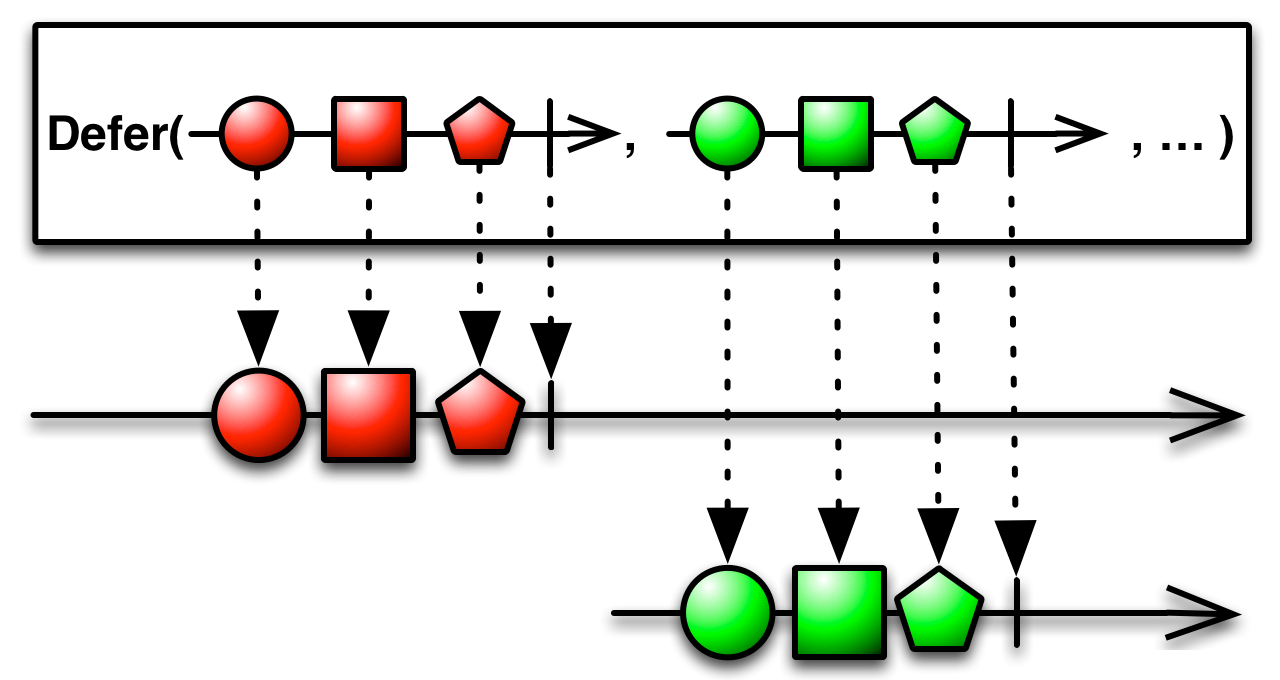
\includegraphics[width=6cm]{defer}
	\caption{Schemat działania operatora Defer}
	\label{defer}
\end{figure}\\
\paragraph{Operatory przekształcania sygnałów}
\subparagraph{Buffer -}cyklicznie zbiera generowane przez obiekt Observable zdarzenia i emituje w postaci pakietów zdarzeń. W przypadku napotkania błędu przez obiekt obserwowany, operator Buffer wyemituje zdarzenie informujące o błędzie bez wytworzenia pakietu danych.
\begin{figure}[ht!]
	\centering
	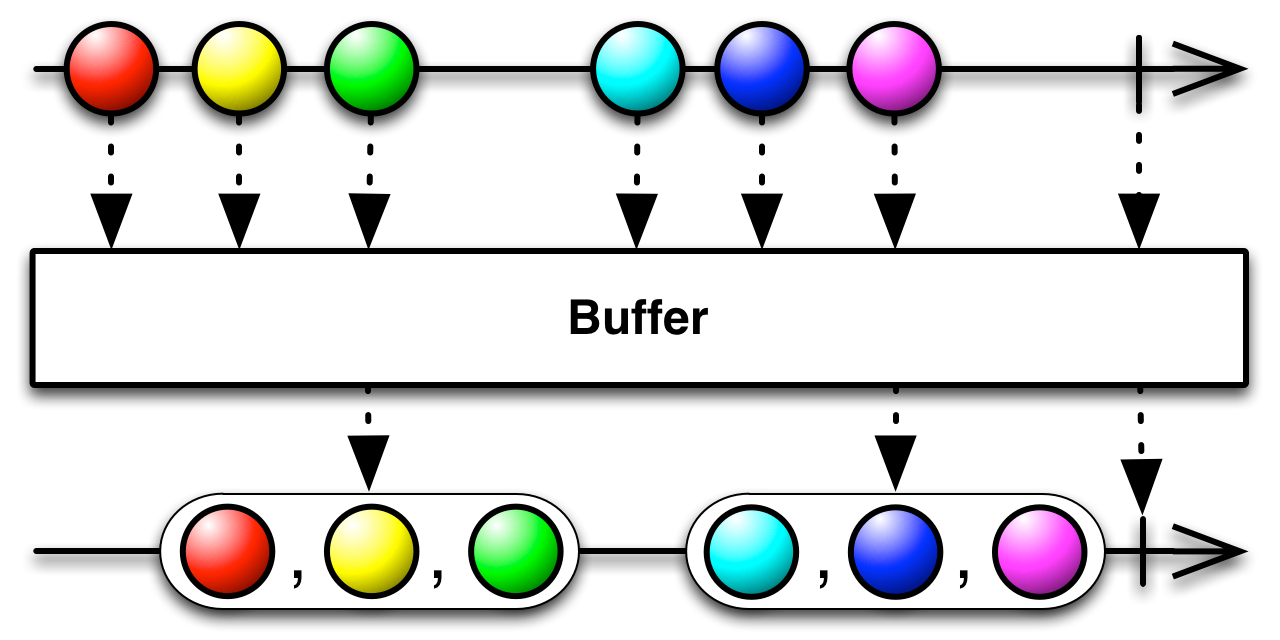
\includegraphics[width=6cm]{buffer}
	\caption{Schemat działania operatora Buffer}
	\label{buffer}
\end{figure}\\
\subparagraph{FlatMap -}przekształca obiekt Observable przez zastosowanie funkcji zdefiniowanej dla każdego wyemitowanego zdarzenia przez źródłowy obiekt obserwowany, gdzie funkcja ta zwraca obiekt Observble emitujący własne zdarzenia. Nastepnie operator flatMap scala emisje wynikowych obiektów Observable w jedną sekwencję danych.
\begin{figure}[ht!]
	\centering
	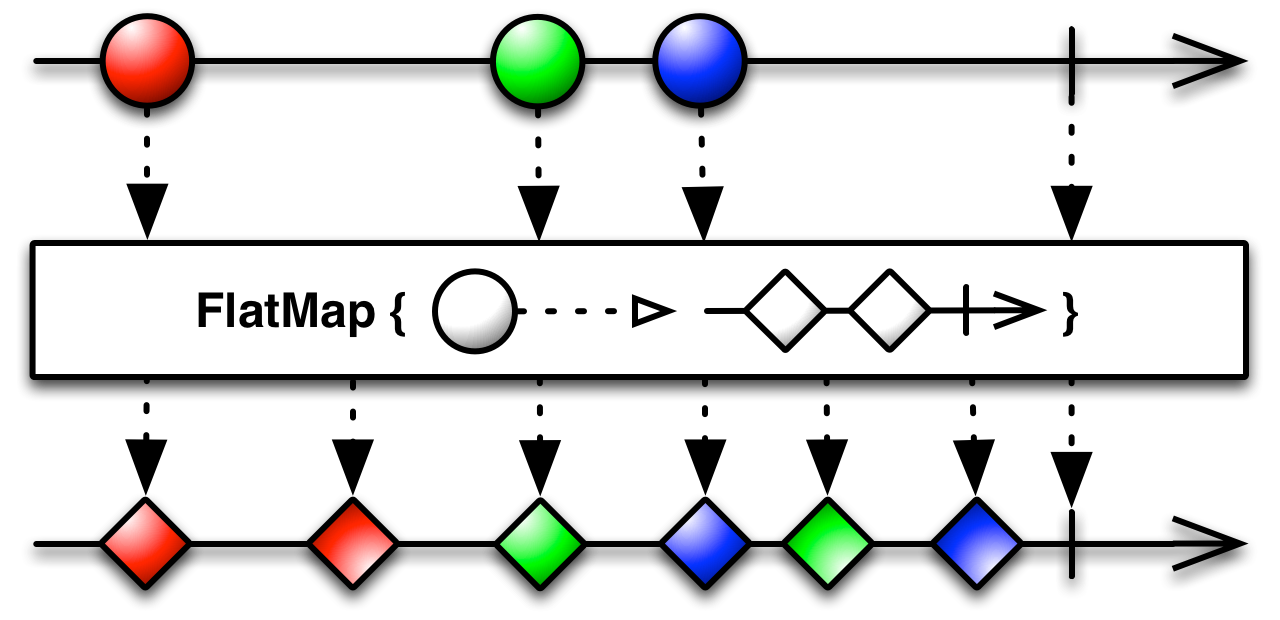
\includegraphics[width=6cm]{flatmap}
	\caption{Schemat działania operatora FlatMap}
	\label{flatmap}
\end{figure}\\
\subparagraph{Map -}stosuje zdefiniowaną funkcję do każdego wyemitowanego przez źródłowy obiekt Observable zdarzenia a następnie zwraca obiekt Observable emitujący przekształcone tą funkcją zdarzenia.
\begin{figure}[ht!]
	\centering
	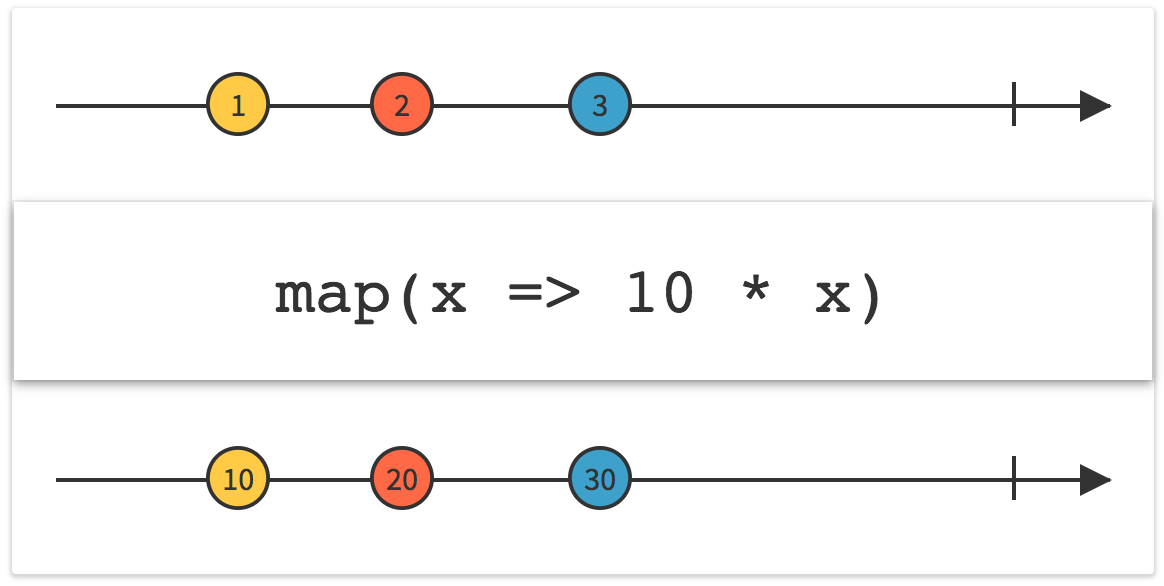
\includegraphics[width=6cm]{map}
	\caption{Schemat działania operatora Map}
	\label{map}
\end{figure}\\
\subparagraph{Scan -}stosuje zdefiniowaną funkcję do pierwszego wyemitowanego przez źródło zdarzenia a następnie emituje to przekształcone zdarzenie jako swoje pierwsze. Wynik tego zdarzenia podawany jest spowrotem to funkcji wraz z kolejnym zdarzeniem z obiektu źródłowego i emitowany.
\begin{figure}[ht!]
	\centering
	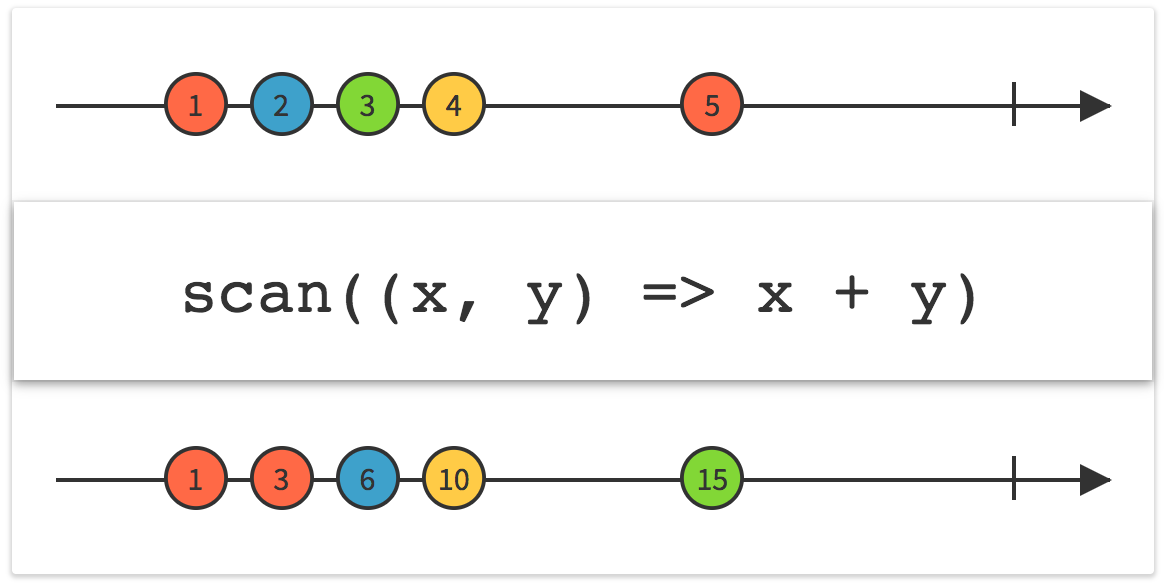
\includegraphics[width=6cm]{scan}
	\caption{Schemat działania operatora Scan}
	\label{scan}
\end{figure}\\
\\
\\
\\
\\
\\
\\
\paragraph{Operatory filtrowania sygnałów}
\subparagraph{Debounce -}emituje zdarzenie z obiektu Observable tylko po upływie zadanego interwału czasowego bez emisji zdarzenia.
\begin{figure}[ht!]
	\centering
	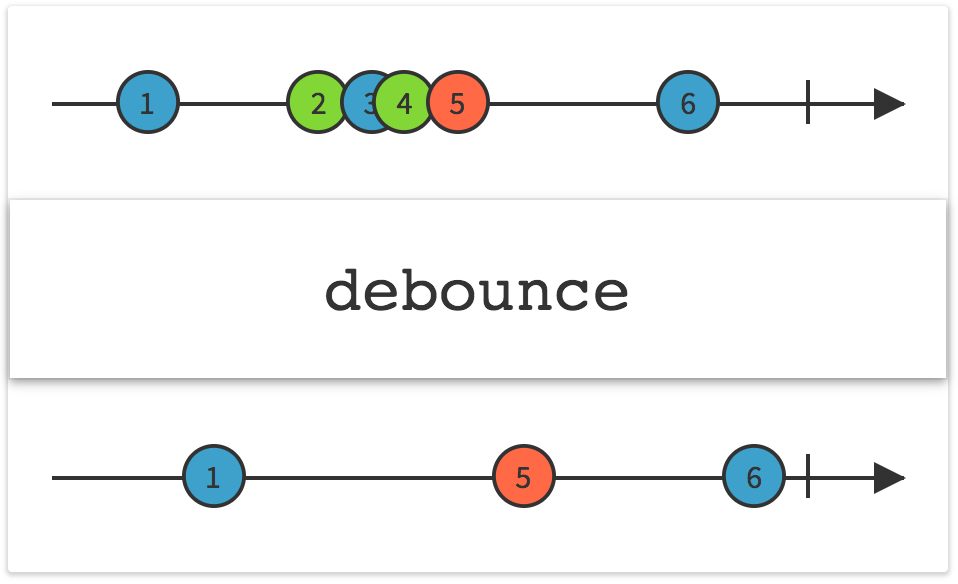
\includegraphics[width=6cm]{debounce}
	\caption{Schemat działania operatora Debounce}
	\label{debounce}
\end{figure}\\
\subparagraph{Distinct -}ignoruje wartości już raz wyemitowane.
\begin{figure}[ht!]
	\centering
	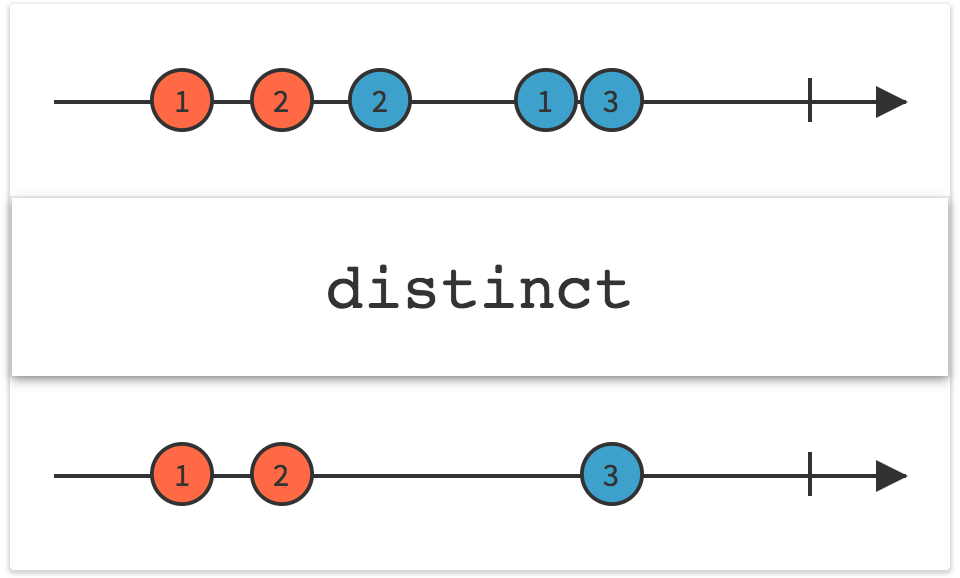
\includegraphics[width=6cm]{distinct}
	\caption{Schemat działania operatora Distinct}
	\label{distinct}
\end{figure}\\
\subparagraph{Filter -}odfiltrowuje zdarzenia emitowane przez obiekt Observable, spełniające wymagania zadanej funkcji lub predykatu.
\begin{figure}[ht!]
	\centering
	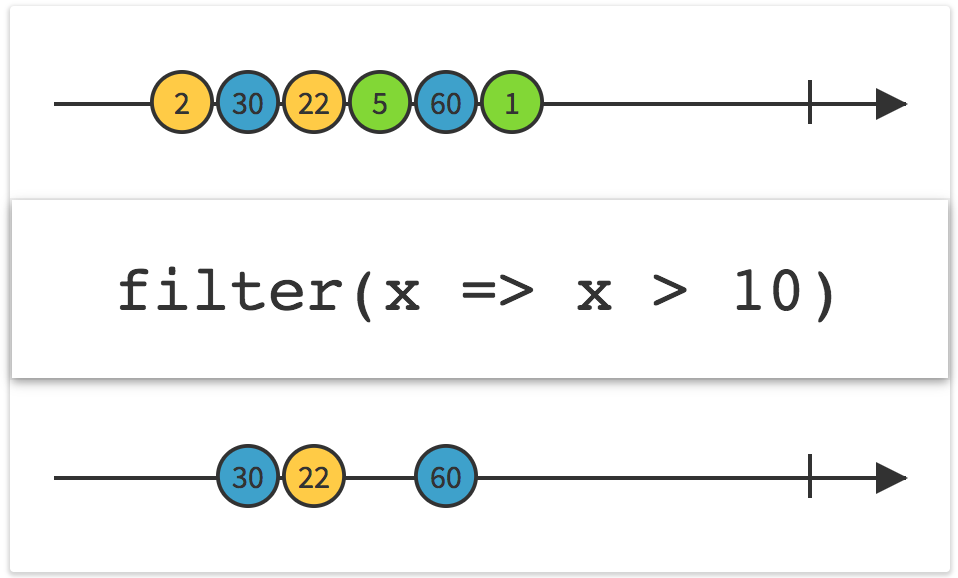
\includegraphics[width=6cm]{filter}
	\caption{Schemat działania operatora Filter}
	\label{filter}
\end{figure}
\subparagraph{Skip -}ignoruje n wygenerowanych przez obiekt Observable zdarzeń, gdzie n jest liczbą naturalną, będącą parametrem.
\begin{figure}[ht!]
	\centering
	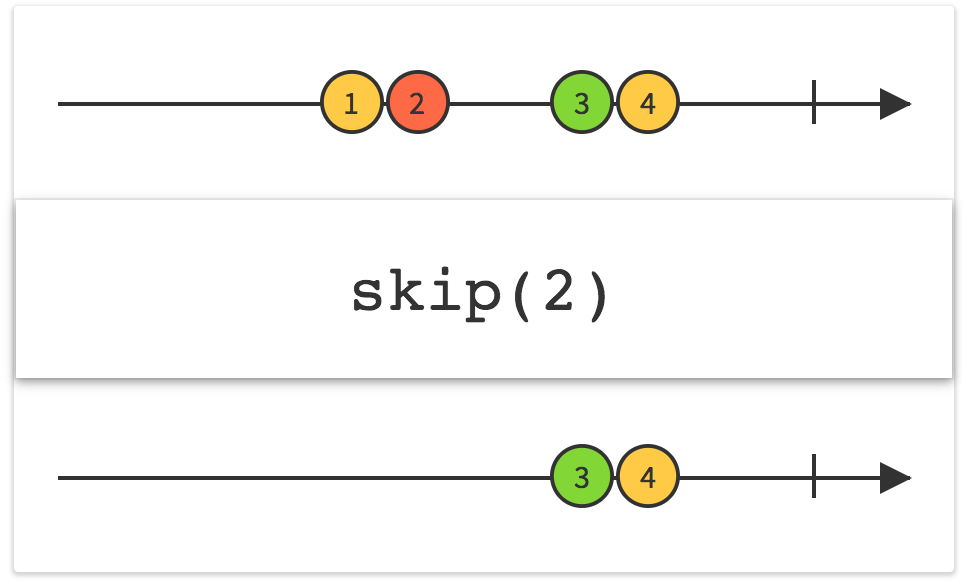
\includegraphics[width=6cm]{skip}
	\caption{Schemat działania operatora Skip}
	\label{skip}
\end{figure}
\subparagraph{Take -}emituje pierwsze n wydarzeń wygenerowanych przez obiekt Observable, gdzie n jest liczbą naturalną, będącą parametrem.
\begin{figure}[ht!]
	\centering
	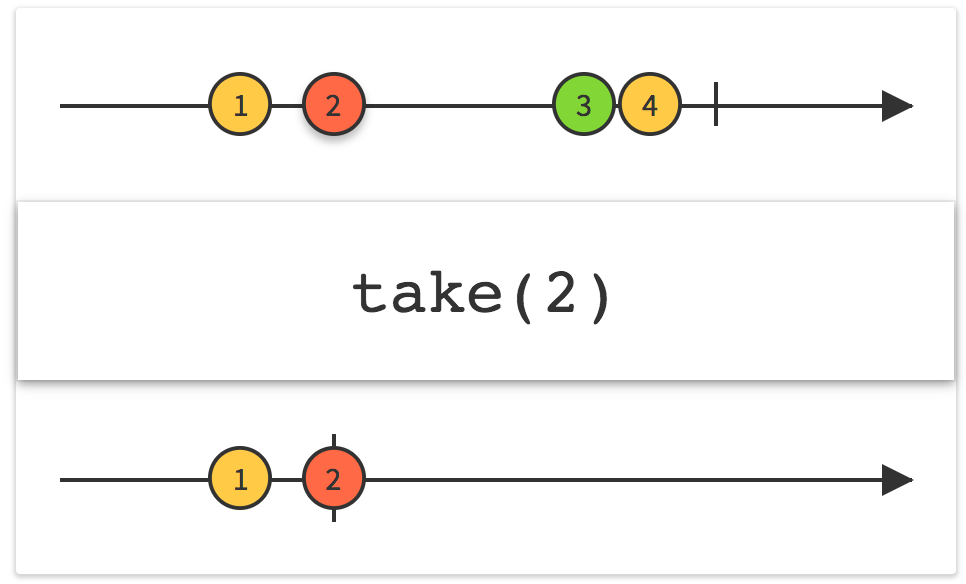
\includegraphics[width=6cm]{take}
	\caption{Schemat działania operatora Take}
	\label{take}
\end{figure}
\paragraph{Operatory łączenia}
\subparagraph{CombineLatest -}łączy ostatnie wyemitowane zdarzenia zadaną funkcją (strategią) z dwóch lub więcej źródeł i emituje nowe zdarzenie będące wynikiem powyższych. 
\begin{figure}[ht!]
	\centering
	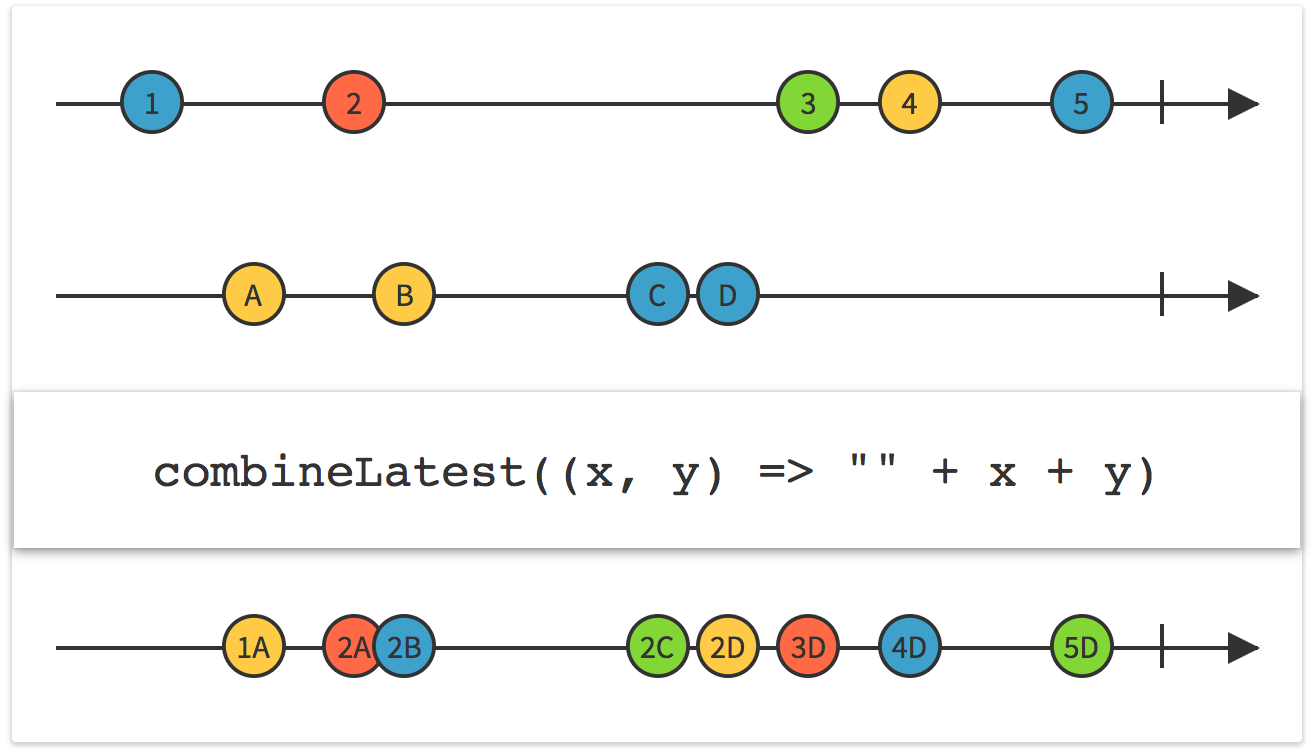
\includegraphics[width=8cm]{combinelatest}
	\caption{Schemat działania operatora CombineLatest}
	\label{combinelatest}
\end{figure}\\
\subparagraph{Merge -}łączy zdarzenia emitowane z wielu sygnałów w jeden ciągły sygnał zdarzeń
\begin{figure}[ht!]
	\centering
	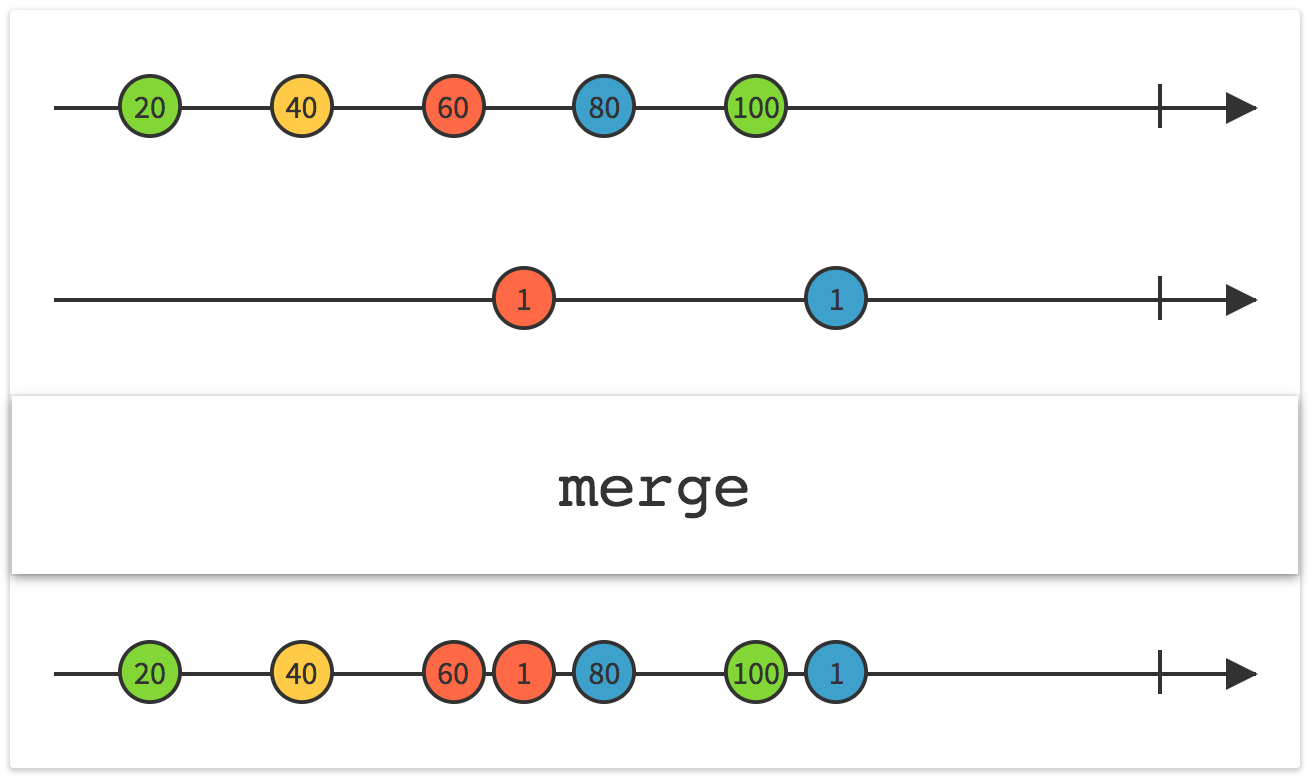
\includegraphics[width=8cm]{merge}
	\caption{Schemat działania operatora Merge}
	\label{merge}
\end{figure}\\
\subparagraph{Zip -}łączy zdarzenia emitowane z dwóch lub więcej sygnałów w pojedyncze zdarzenia reprezentowane krotką. 
\begin{figure}[ht!]
	\centering
	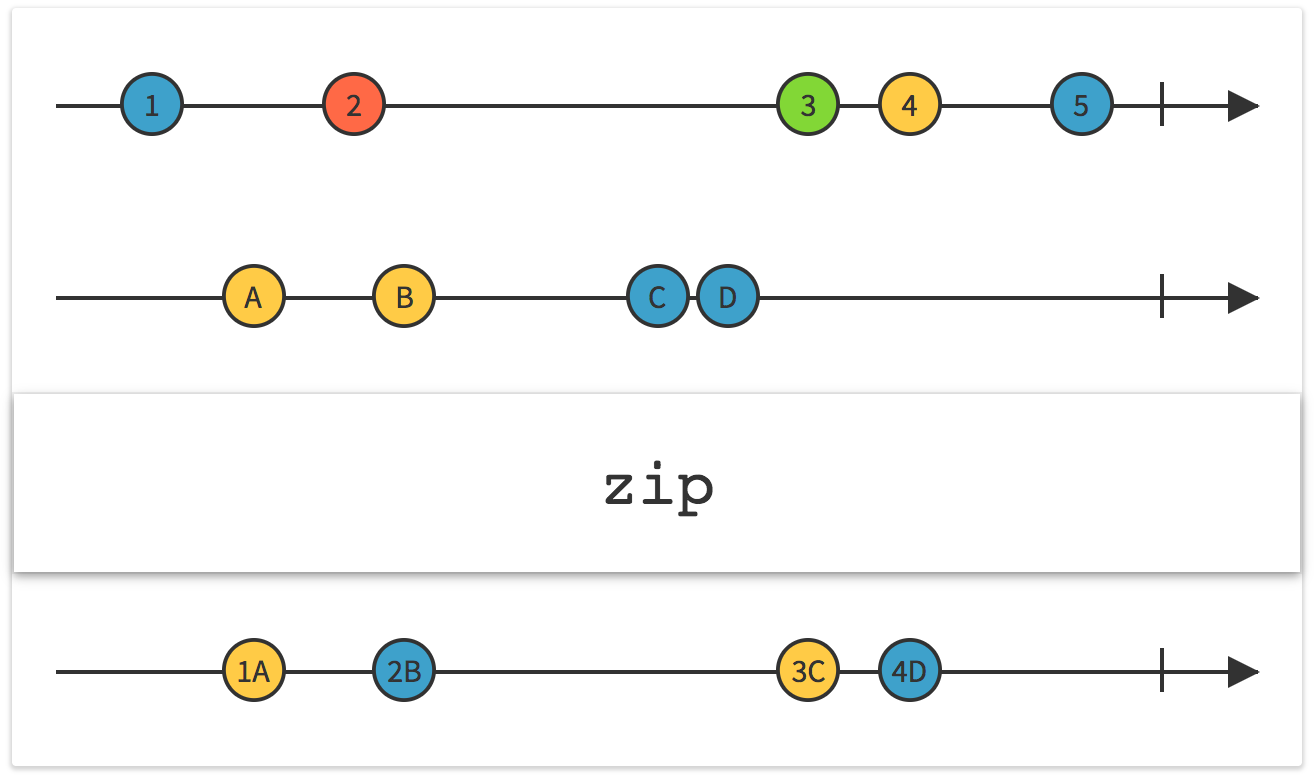
\includegraphics[width=8cm]{zip}
	\caption{Schemat działania operatora Zip}
	\label{zip}
\end{figure}\\
\\
\\
\subsection{Współbieżność}
\subsection{Wady i zalety podejścia reaktywnego} 
\subsection{Implementacja na platformie iOS}
\chapter{PRACA WŁASNA}
\section{Czynności przygotowawcze}		
\paragraph{}Stworzenie aplikacji mobilnej było możliwe dzięki wykonaniu uprzednio czynności przygotowawczych. Do czynności tych należało: wybór środowiska programistycznego, instalacja bibliotek i frameworków, wstępna konfiguracja projektu oraz stworzenie repozytorium.
\subsection{Instalacja narzędzi}
\paragraph{}Program XCode jest jednym z niewielu dostępnych środowisk programistycznych na platformę iOS. Jest on darmowy i dostarczany wraz systemem MacOS. XCode posiada wbudowany kompilator LLVM oraz szereg przydatnych narzędzi tj. interface builder - graficzny edytor do tworzenia elementów interfejsu, dynamiczną kontrolę składni czy menedżer systemu kontroli wersji. Ze względu na powyższe właściwości zdecydowałem się użyć właśnie tego środowiska programistycznego.
Ponadto użyłem także narzędzia do rozwiązywania zależności - CocoaPods. Jest ono bardzo przydatne szczególnie przy instalacji bibliotek i frameworków do projektu.  
\subsection{Wstępna konfiguracja projektu}
\paragraph{}Podczas konfigurowania projektu w środowisku XCode istotne jest abyśmy stworzyli go z użyciem CoreData. Jest to baza danych środowiska iOS i może stanowić integralną część aplikacji.   
\subsection{Stworzenie repozytorium}
\paragraph{}Dostępnych jest wiele systemów kontroli wersji, ale najpopularniejszym z nich jest GIT. Zdecydowałem się na jego wykorzystanie, ponieważ jest dosyć prosty w użyciu a większość serwerów GITa jest darmowa. Użycie systemu typu GIT pozwoli mi na kontrolę postępów mojej pracy jak i na dokumentowanie jej. Oprócz tego użycia GITa powoduje, że błąd popełniony przeze mnie na dalszym etapie mogę odwrócić przywracając poprzedni stan projektu.
\section{Budowa aplikacji właściwej}
\subsection{Wymagania funkcjonalne}
\subsection{Wymagania niefunkcjonalne}
\subsection{Diagram przypadków użycia aplikacji}
\subsection{Zależności w bazie danych}
\subsection{Diagram klas}
\subsection{Opis wybranych klas}
\subsection{Opis użytych bibliotek i frameworków}
\subsection{Implementacja aplikacji mobilnej - zastosowana architektura}
\subsection{Prezentacja aplikacji}
\begin{thebibliography}{50}
\bibitem{MicrosoftRx} https://msdn.microsoft.com/en-us/library/hh242985(v=vs.103).aspx
\emph{- informacje na temat Reactive Extensions od Microsoft}
\bibitem{swiftHistory} https://developer.apple.com/swift/blog/?id=14
\emph{- historia języka Swift}
\bibitem{swiftOpensource} https://developer.apple.com/swift/blog/?id=34
\emph{- Swift jako język opensource}
\bibitem{swiftObjcDiff} https://redwerk.com/blog/10-differences-objective-c-swift
\emph{- Różnice między Swiftem a Objective - C}
\bibitem{pureDarwin} www.puredarwin.com 
\emph{ - informacje o systemie Darwin}
\bibitem{openGroup} www.opengroup.org \emph{ - informacje o systemach unixowych}
%\bibitem{XNUkernel} https://developer.apple.com/library/content/documentation/MacOSX/Conceptual/OSX_Technology_Overview/SystemTechnology/SystemTechnology.html#//apple_ref/doc/uid/TP40001067-CH207-BCICAIFJ
%\emph{ - opis jądra systemu MacOS i iOS}
%\bibitem{iphoneOSX} https://web.archive.org/web/20071006005308/http://www.apple.com/iphone/features/index.html#macosx
%\emph{ - informacje o pierwszym systemie na iPhone}
\bibitem{iphoneSDK} https://web.archive.org/web/20071020040652/http://www.apple.com/hotnews
\emph{ - informacja o stworzeniu i udostępnieniu iPhone SDK}
\bibitem{iphone3GappStore} http://www.apple.com/pr/library/2008/07/10iPhone-3G-on-Sale-Tomorrow.html
\emph{ - informacje o iPhone 3G i powstaniu usługi App Store}
\bibitem{iphoneOS3} http://www.apple.com/pr/library/2009/06/08Apple-Announces-the-New-iPhone-3GS-The-Fastest-Most-Powerful-iPhone-Yet.html
\emph{ - system iPhone 3.0 i implementacja podstawowych funkcjonalności}
\bibitem{ios4}http://www.apple.com/pr/library/2010/04/08Apple-Previews-iPhone-OS-4.html
\emph{ - informacje o systemie iOS 4}
\bibitem{ios5}http://www.apple.com/pr/library/2011/10/04Apple-Launches-iPhone-4S-iOS-5-iCloud.html
\emph{ - informacje o systemie iOS 5}
\bibitem{ios6}http://www.apple.com/pr/library/2012/06/11Apple-Previews-iOS-6-With-All-New-Maps-Siri-Features-Facebook-Integration-Shared-Photo-Streams-New-Passbook-App.html
\emph{ - informacje o systemie iOS 6}
\bibitem{ios7}http://www.apple.com/pr/library/2013/06/10Apple-Unveils-iOS-7.html
\emph{ - informacje o systemie iOS 7}
\bibitem{ios8}http://www.apple.com/pr/library/2014/06/02Apple-Releases-iOS-8-SDK-With-Over-4-000-New-APIs.html
\emph{ - informacje o systemie iOS 8}
\bibitem{ios9}http://www.apple.com/pr/library/2015/06/08Apple-Previews-iOS-9.html
\emph{ - informacje o systemie iOS 9}
\bibitem{compatibility}https://github.com/apple/swift-evolution/blob/master/proposals/0005-objective-c-name-translation.md
\emph{ - informacje o poprawieniu kompatybilności Swift z Objective-C}
\bibitem{ios10}http://www.apple.com/pr/library/2016/06/13Apple-Previews-iOS-10-The-Biggest-iOS-Release-Ever.html
\emph{ - informacje o systemie iOS 10}
\bibitem{beginningOfRx} Czaplicki, Evan (Apr 2012), Elm: Concurrent FRP for Functional GUIs (PDF) (thesis), Harvard
\emph{ - pierwsze wzmianki o programowaniu reaktywnym}
\bibitem{rxMicrosoftYear} http://www.introtorx.com/content/v1.0.10621.0/00foreword.html
\emph{ - wypuszczenie biblioteki Reactive Extensions}
\bibitem{rxDesignGuideline} https://go.microsoft.com/fwlink/?LinkID=205219
\emph{ - wytyczne projektowe paradygmatu reaktywnego}
\end{thebibliography}
\chapter{PODSUMOWANIE}

\end{document}          
